\chapter{Ray Tracing}
\label{chap:ray-tracing}

There exists several methodologies to solve the neutron transport equation for a particular reactor geometry and material composition. Each methodology involves a different set of assumptions that can be applied to the neutron transport equation in order to simplify it into a form that can be solved numerically. The Method of Characteristics (MOC) approach solves the equation along characteristic tracks, across which the solution of the angular flux reduces to an ordinary differential equation. The scalar flux in a given region, which is necessary to calculate reaction rates, can be calculated by summing the contributions from each track's angular flux through the region. Often the approximation of a constant neutron source in each source region is applied, although higher order solutions exist. This flat source approximation leads to a simple exponential attenuation of the angular flux, $\psi$, through the flat source region (FSR) given in Eq.~\ref{eq::fsr_attenuation}

\begin{equation}
\psi(s) = \psi(0) e^{-\Sigma_t s} + \frac{q}{\Sigma_t} \left( 1 - e^{-\Sigma_t s} \right)
\label{eq::fsr_attenuation}
\end{equation}

where $\Sigma_t$ is the total cross-section, $s$ is the distance the track travels through the FSR, and $q$ is the constant neutron source in the FSR. With this approximation, the scalar flux, $\phi$, in a given FSR can be calculated by summing the contributions of each angular flux, as is given in Eq.~\ref{eq::scalar_flux}

\begin{equation}
\phi = \frac{4\pi}{\Sigma_t} \left(q + \frac{1}{V} \sum_{k\in V} w_k \Delta \psi_k \right)
\label{eq::scalar_flux}
\end{equation}

where $w_k$ is the weight of track $k$, $\Delta \psi_k$ is the change in the angular flux of track $k$ over the FSR, and $V$ is the volume of the FSR.

These equations are most widely applied in 2D, where the volume transforms to an area and tracks are laid down in 2D. In this scheme a certain polar quadrature is used so that for each 2D track, multiple angular fluxes are represented across both polar angle and neutron energy group. In 3D MOC, the tracks are explicitly laid across the 3D geometry so that each track represents a specific polar angle, although each track still represents multiple angular fluxes across energy groups. 

The first step of standard MOC solvers is to lay tracks across the geometry. During this procedure, tracks connect with complementary tracks to satisfy boundary conditions. The tracks' spacings and angles are modified to ensure every track exactly intersects with a complementary track at the boundaries. While simple in theory, this procedure can result in unnecessary modifications to the tracks' spacings and angles that can significantly increase the memory and compute requirements of the problem \cite{sam_old}. The track generation procedure is typically done in a piecewise manner. First, 2D tracks are laid down in the x-y plane according to a procedure described by Filippone \cite{filippone}. Next, 3D tracks are laid down on top of the 2D tracks following one of several procedures: Modular Ray Tracing, simplified-Modular Ray Tracing, and 3D Global Tracking \cite{sam_old, kochunas}. Groups of tracks sharing the same 2D track and polar angle are denoted as $z-$stacks in this paper. A depiction is shown in Fig.~\ref{fig::3D_tracks}.

\begin{figure}[ht!]
	\centering
	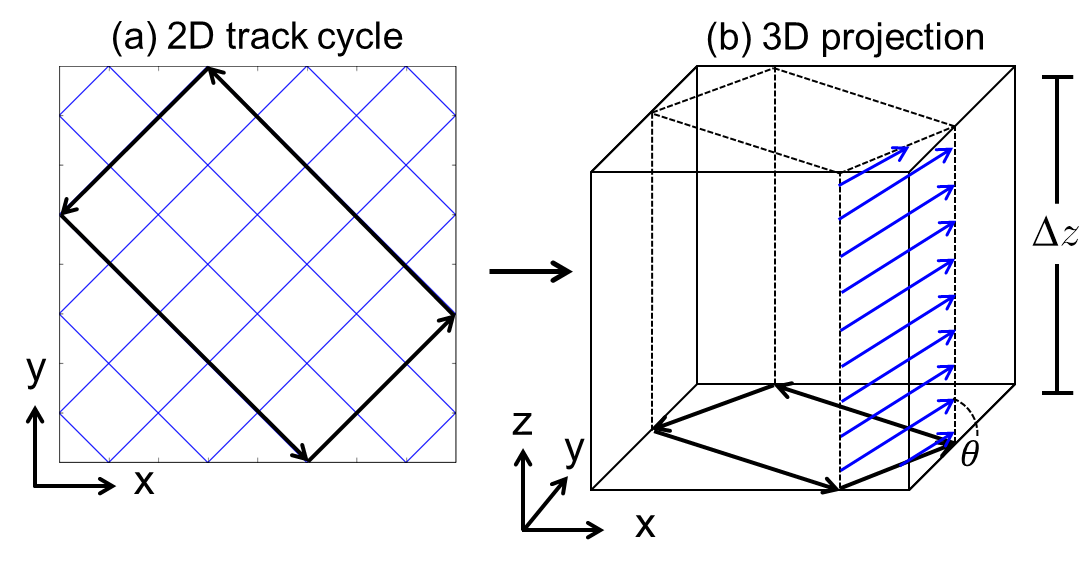
\includegraphics[width=0.75\linewidth]{figures/ph2016/3DMOC_stack.png}
	\caption{Depiction of creating $z$-stacked tracks given a polar angle $\theta$ and a 2D track.}
	\label{fig::3D_tracks}
\end{figure}

Once the tracks are laid across the geometry, they are partitioned by source region intersections into segments (or crossings) across which the MOC equations can be applied. For simplicity, we will assume in this paper all source regions are spatially flat and will hereafter denote a flat source region as an FSR. At a minimum, the segment lengths and associated FSR identifiers are saved for each track. After this is completed, the sweeping process starts in which Eq.~\ref{eq::fsr_attenuation} and Eq.~\ref{eq::scalar_flux} are applied to all segments with some initial guess of scalar fluxes and boundary angular fluxes. 

%This describes the common implementation of 2D MOC. The simple extension of this implementation to 3D MOC is presented in Algorithm~\ref{alg::old}.

%\begin{algorithm*}[!h]
%\caption{3D MOC algorithm extending the standard 2D approach}
%\label{alg::old}
%\begin{algorithmic}
%\STATE User specifies materials and a geometry
%\STATE Generate tracks across the geometry
%\FORALL{$i \in \text{2D tracks}$}
%  \FORALL{$\theta \in \text{polar angles}$}
%    \FORALL{$t \in \text{z-stack for 2D track } i \text{ and polar angle } \theta$} 
%        \STATE Segment track $t$ into segments, saving the segment lengths and corresponding FSR identifiers, populating 3D FSRs as new regions are traversed
%    \ENDFOR
%  \ENDFOR
%\ENDFOR
%\FORALL{transport sweeps}
%    \FORALL{$i \in \text{2D tracks}$}
%      \FORALL{$\theta \in \text{polar angles}$}
%        \FORALL{$t \in \text{z-stack for 2D track } i \text{ and polar angle } \theta$}
%            \FORALL{$s \in \text{segments for track } t$}
%                \STATE Apply Eq.~\ref{eq::fsr_attenuation} and Eq.~\ref{eq::scalar_flux} to segment $s$ and the corresponding FSR
%                \ENDFOR
%            \ENDFOR
%        \ENDFOR
%    \ENDFOR
%    \IF{Source is converged} 
%        \RETURN
%    \ENDIF
%\ENDFOR
%\end{algorithmic}
%\end{algorithm*}

While this approach is straightforward, its memory and compute requirements for 3D MOC can be prohibitive, even for small problems. Reducing the memory footprint is important for many reasons. Recently, the Chord Classification Method (CCM) \cite{Sciannandrone2015} was presented for axially extruded geometries to reduce memory requirements by only saving the unique chords (or segments).  However, this method still requires that the segmentation procedure be performed for all 3D tracks prior to performing transport sweeps, which can be prohibitively expensive for complex geometries. In this study, an alternative approach is presented that utilizes some ideas of CCM and greatly reduces the segment storage and generation requirements by taking advantage of the extruded geometry structure common to many reactor physics problems.

\section{METHODOLOGY}

An important observation of nuclear reactor cores is their close resemblance to axially extruded geometries. Here, an axially extruded geometry is defined to be a geometry in which every radial slice of the reactor geometry is identical. Note this is a requirement only on the radial geometry, not the materials. Given an axially extruded geometry, it is possible to store only the 2D segments associated with intersections in the radial geometry. The 3D segments can then be formed on-the-fly using a simple axial mesh.

\subsection{Forming an Axially Extruded Geometry}

While common reactor cores contain variations from axially extruded geometries, such as end plugs for control rods, most of these variations can be fully captured at little cost by implicitly inserting additional geometric regions.

First, 2D segments need to be formed which reflect intersections of the 2D tracks with a superposition of all radial surfaces in the geometry. This is done by simultaneously ray tracing across all the unique radial planes in the geometry, as depicted in Fig.~\ref{fig::superposition}. This creates an implicit geometry containing all radial information, which we refer to as the superposition plane. The 2D geometric regions in the superposition plane correspond to an axially extruded region with an associated unique identifier that contains an axial mesh and an array of associated 3D FSRs. 

\begin{figure}[ht!]
	\centering
	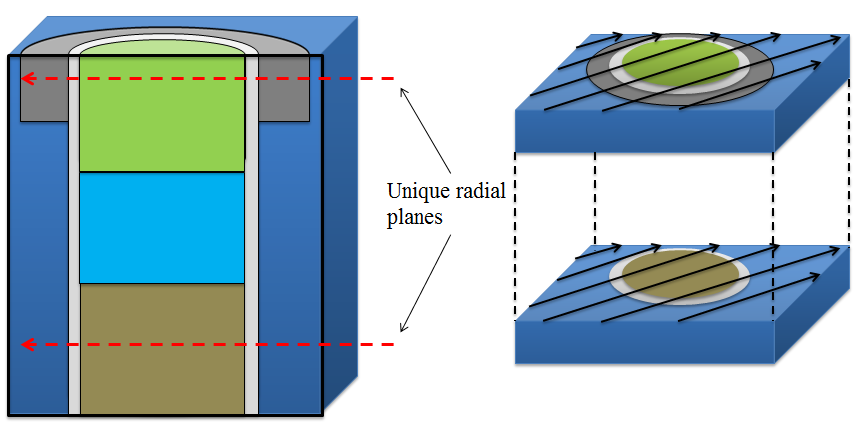
\includegraphics[width=\linewidth]{figures/ph2016/new_unique_z_levels_v_extruded_rt2.png}
	\caption{Depiction of 2D ray tracing for superposition of all radial detail.}
	\label{fig::superposition}
\end{figure}

Each 2D segment formed during the ray tracing contains its length and the unique identifier of the axially extruded region being traversed. After 2D segmentation, axial meshes need to be created for on-the-fly axial ray tracing. If a global axial mesh is desired, whereby all axially extruded regions have the same axial mesh, all the unique z-planes in the geometry are collected and sorted into an axial mesh. Otherwise, local meshes are populated for each axially extruded region during population of the 3D FSRs. To populate the 3D FSRs, a temporary vertical ray is created for each axially extruded region. These rays all start from the bottom of the root geometry and are directed upwards and segmented to determine distances between axial intersections and initialize the associated FSR.

Implicitly, this strategy can create extra radial intersections since some of the axial levels might not have originally contained the full radial detail of the superposition plane. However, the number of additional intersections should be low due to the regular structure of most reactor cores. For instance, fuel rods with end plugs present only a slight deviation from an axially extruded geometry.

The advantage of local axial meshes is the ability to have different axial refinements within the reactor. For instance, a partially inserted control rod might need a finer FSR discretizations near the control rod tip. If a global axial mesh were used, the finer discretization would need to be applied to the whole core at that axial height, including the reflector. With local axial meshes, only the regions which need refinement would use a finer discretization.

\subsection{On-the-fly Axial Ray Tracing}

During the transport sweeps, each 3D track is traversed until it reaches its end point on a geometry bounding surface. The common method presented in section~\ref{sect::intro} accomplishes this by splitting every 3D track into 3D segments before the transport sweeps and then simply cycling through all the segments of the track sequentially.

In the methods presented here, 3D segments are recreated on-the-fly for each 3D track using information stored in the 2D tracks formed during initial ray tracing. Due to the manner in which the 3D tracks were formed, each 3D track corresponds to one of the segmented 2D tracks. From the starting locations and polar angles, it is possible to determine the distance along the track to an axial intersection using an axial mesh and to a radial intersection using the 2D segments. On-the-fly axial ray tracing can either be performed on each 3D track individually or on a whole $z$-stack.

\subsubsection{Ray Tracing Individual 3D Tracks}


\begin{figure}[ht!]
	\centering
	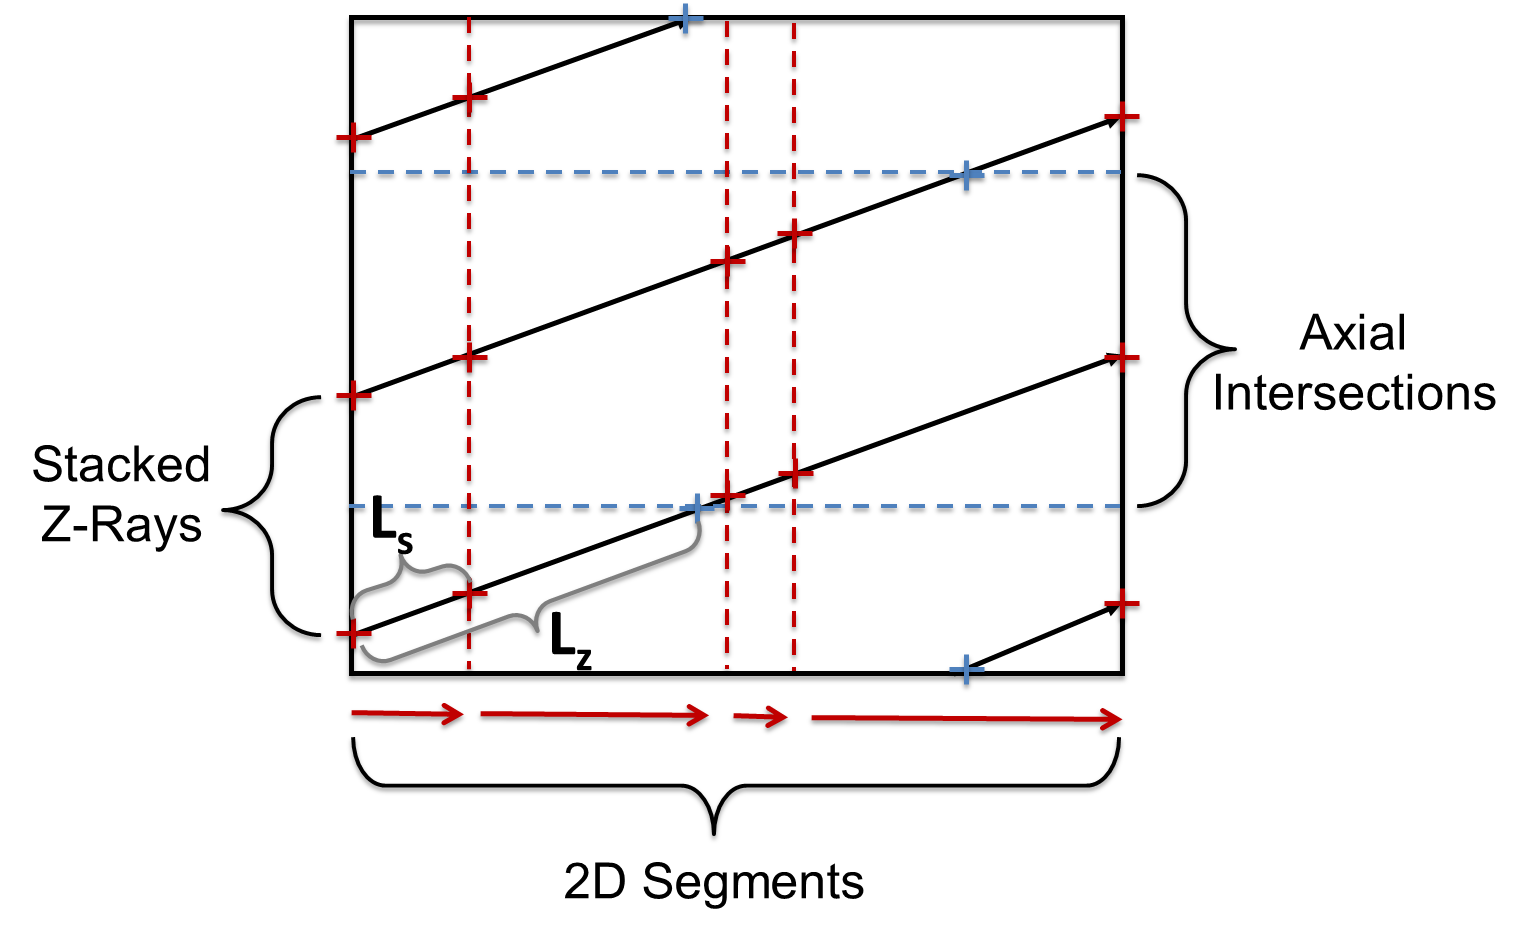
\includegraphics[width=0.75\linewidth]{figures/ph2016/otf_ray_tracing.png}
	\caption{Illustration of the on-the-fly axial ray tracing process with axial intersections colored in blue and radial intersections colored in red. For the chosen track, the distance to the next axial intersection is denoted $L_z$ and the the distance to the next radial intersection is denoted $L_s$.}
	\label{fig::otf_ray_tracing}
\end{figure}



For ray tracing each 3D track individually, the associated 2D segments are traversed until the 3D track reaches its endpoint. First, the starting point is used to determine the appropriate starting 2D segment and index into the axial mesh. If local meshes are used, the index needs to be recomputed with a binary search at the start of each 2D segment. If a global mesh is used, the axial index only needs to be calculated at the beginning of the track. The 2D segments are traversed and the shorter distance to either an axial or radial intersection is calculated. This computed distance is the 3D segment length and has an associated 3D FSR indicated by the axial index. To form the next 3D segment, the position along the 2D track is moved by the appropriate distance. This process is repeated until the endpoint is reached. An illustration of this concept is presented in Fig.~\ref{fig::otf_ray_tracing}.

\subsubsection{Ray Tracing 3D Track Z-Stacks}

The structure of the 3D track laydown can be used to ray trace an entire $z$-stack. Specifically all tracks in the $z$-stack have the same polar angle $\theta$, project onto the same 2D track, and are separated by a constant axial ray spacing $\Delta z$. Therefore, if we define $z_0(0)$ as the $z$-coordinate at the intersection of the lowest track with the $z$-axis at the start of the associated 2D track, the axial height $z_i$ of the $i^{\textit{th}}$ lowest track (starting from 0) can be defined as

\begin{equation}
z_i(s) = z_0(0) + i\Delta z + s \cot{\theta}
\label{eq::track_projection}
\end{equation}

where $s$ is the distance along the associated 2D track. Combining this with 2D track information is enough to completely describe the trajectory and location of 3D tracks in the stack. Therefore, it is possible to determine which tracks will traverse a given FSR.

For each 2D segment in the 2D track, there is an associated axially extruded region which contains a list of 3D FSRs in the region. To trace a $z$-stack, intersections within axially extruded FSRs are determined in the order traversed by the 2D segments. The 1D axial mesh (either local or global) associated with the axially extruded region is used to determine the axial boundaries of each 3D FSR. Using the boundaries of the FSR and Eq.~\ref{eq::track_projection}, it is possible to analytically compute the indexes of tracks that will cross the FSR as

\begin{equation}
%i_\textit{start} = \ceil[\Big]{\frac{z_\textit{min} - \max\left({z_0(s_\textit{start}), z_0(s_\textit{end}})\right) }{\Delta z}}
FIXME
\label{eq::start_track}
\end{equation}

\begin{equation}
%i_\textit{end} = \floor[\Big]{\frac{z_\textit{max} - \min\left({z_0(s_\textit{start}), z_0(s_\textit{end}})\right) }{\Delta z}}
FIXME
\label{eq::end_track}
\end{equation}


where $i_{\textit{start}}$ is the index of the first track to cross the FSR, $i_{\textit{end}}$ is the index of the last track to cross the FSR, $s_{\textit{start}}$ is the 2D distance traversed at the start of the segment and $s_{\textit{end}}$ is the 2D distance traversed at the end of the segment. A depiction of this process is shown in Fig.~\ref{fig::stack_tracing}.

\begin{figure}[ht!]
	\centering
	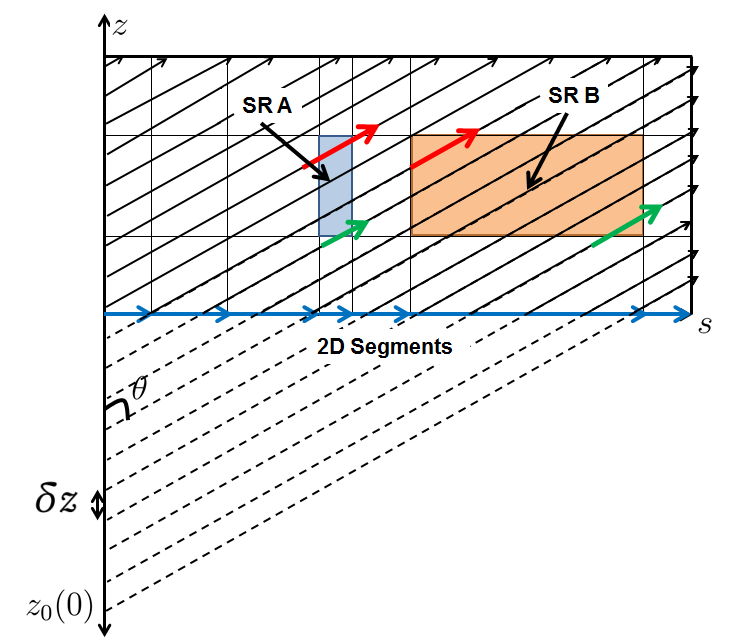
\includegraphics[width=0.75\linewidth]{figures/ph2016/stack_tracing.png}
	\caption{Illustration of the on-the-fly axial ray tracing process for an entire $z$-stack. The green arrows denote the first track to traverse the highlighted FSRs calculated by Eq.~\ref{eq::start_track} and the red arrows denote the last tracks to traverse the FSRs calculated by Eq.~\ref{eq::end_track}.}
	\label{fig::stack_tracing}
\end{figure}


Notice that for FSR A depicted in Fig.~\ref{fig::stack_tracing} there are multiple track segments that cross the entire 2D length of the FSR and are therefore identical. Their 3D segment length $L_{3D}$ would simply be
\begin{equation}
L_{3D} = \frac{s_{\textit{end}} - s_{\textit{start}}}{\sin{\theta}}.
\end{equation}

In common reactor physics problems we expect this effect to be much more pronounced. Due to the radial direction having much greater complexity than the axial direction, FSRs will tend to be longer in the axial direction than in the radial plane, especially when higher order sources are added in the axial direction. The high aspect ratio would cause many tracks to cross the entire 2D length of the FSR.

To take advantage of this, it is possible to calculate the indexes of the first and last tracks to traverse the entire 2D segment length. For this condition to be met, the axial height of the tracks over the entire 2D segment must be greater than the minimum axial boundary of the FSR and less than the maximum axial boundary. Therefore, the indexes of interest are the first track to have its lowest point above the minimum boundary and the first track to have its highest point above the maximum boundary. We name this indexes $i_{\textit{in}}$ and $i_{\textit{out}}$ respectively and they can be calculated as:

\begin{equation}
%i_{\textit{in}} = \ceil[\Big]{\frac{z_\textit{min} - \min\left({z_0(s_{\textit{start}}), z_0(s_{\textit{end}}})\right) }{\Delta z}}
FIXME
\end{equation}

\begin{equation}
%i_{\textit{out}} = \ceil[\Big]{\frac{z_\textit{max} - \max\left({z_0(s_{\textit{start}}), z_0(s_{\textit{end}}})\right) }{\Delta z}}
FIXME
\end{equation}

For each FSR these indexes are calculated along with those beginning and end track indexes given in Eq.~\ref{eq::start_track} and Eq.~\ref{eq::end_track}. It is possible that $i_{\textit{in}}$ will be greater than $i_{\textit{out}}$ when the polar angle is steep enough, allowing for the FSR to be fully traversed axially without traversing the entire 2D length. These tracks can be determined with indexes $i_{\textit{in}}$ and $i_{\textit{out}}$ and have a common 3D segment length $L_{3D}$ given by
\begin{equation}
L_{3D} = \frac{z_{\textit{max}} - z_{\textit{min}}}{\left| \cos{\theta}\right|}.
\end{equation}

Therefore, 3D segments are classified into four categories:

\begin{itemize}
	\item \textbf{Mixed Tracks -- Case A:} Tracks that partially traverse the FSR and cross the lower FSR boundary. They are defined by track indexes $i_{\textit{start}} \leq i < \min\left(i_{\textit{in}}, i_{\textit{out}}\right)$. For these tracks, each 3D segment is computed individually. 
	\item \textbf{Mixed Tracks -- Case B:} Tracks that partially traverse the FSR and cross the upper FSR boundary and each 3D segment is again computed individually. They are defined by track indexes $\max\left(i_{\textit{in}}, i_{\textit{out}}\right)  \leq i  \leq i_{\textit{end}}$`
	\item \textbf{Horizontal Tracks:} Tracks that fully traverse the entire 2D radial distance of the FSR and are defined by indexes $i_{\textit{in}} \leq i < i_{\textit{out}}$. 
	\item \textbf{Vertical Tracks:} Tracks that traverse the entire axial distance of the FSR and are defined by $i_{\textit{out}} \leq i < i_{\textit{in}}$.
\end{itemize}

\subsection{Applying the MOC Equations}
The 3D segments that are computed from the axial on-the-fly ray tracing can either be stored in temporary arrays of segments or directly used to apply Eq.~\ref{eq::fsr_attenuation} to the associated track's angular flux and Eq.~\ref{eq::scalar_flux} to the associated FSR as they are formed. In MOC, it is common to have each track represent both a forward and backward angular flux to maximize efficiency and reduce the amount of book keeping associated with each angular flux. 

The advantage to temporarily storing segments is that ray tracing would only need to be performed in the forward direction along each track. Once the segments are stored in the temporary arrays, the MOC equations presented in Eq.~\ref{eq::fsr_attenuation} and Eq.~\ref{eq::scalar_flux} can be applied forward to the stored segments and then backward, representing the forward and backward angular fluxes. The temporary arrays are created at the beginning of the solver. For on-the-fly axial ray tracing by individual 3D track, one temporary array of segments needs to be created of size $S$ equal to the maximum number of segments per 3D track. For on-the-fly axial ray tracing by $z$-stack, the $M$ temporary arrays of segments need to be created of size $S$ where $M$ is the maximum number of tracks per $z$-stack.

Alternatively, if the segments are used in Eq.~\ref{eq::fsr_attenuation} and Eq.~\ref{eq::scalar_flux} immediately after formation, ray tracing needs to be performed both forward and backward along the tracks. This additional ray tracing cost should make this alternative method more expensive for ray tracing by individual 3D tracks. However for ray tracing by $z$-stacks, there will be increased cache efficiency from tracks that tally scalar flux contributions to the same FSR. In practice, FSRs are allocated continuously in memory by axial level so there is the potential of cache reuse from this method coupled with ray tracing by $z$-stacks. Because of this reasoning, results will only be shown for this method tested with ray tracing by $z$-stacks.

\section{RESULTS}

The methods described above were implemented into OpenMOC\cite{openmoc}, an open source MOC solver. Performance results are presented for the OpenMOC solver with the various different ray tracing schemes. All performance results were gathered from jobs submitted on Amazon Web Services' (AWS) Elastic Compute Cloud (EC2) on m4.10xlarge nodes which each have 40 CPU cores and 160 GB RAM.

\subsection{Description of Test Problem}
To test the different approaches to 3D MOC segment formation, a single test problem is chosen to represent the type of geometries encountered in reactor core simulations. Specifically, the central UO$_{\text{2}}$ assembly of the 3D C5G7 Benchmark Unrodded geometry was used with reflective boundaries on all surfaces except the top axial surface, which has a vacuum boundary. A detailed description of additional test problem parameters is given in Table~\ref{tab::problem}.

\begin{table}[ht]
	\centering
	\caption{Test Problem Parameters}
	\medskip
	\begin{tabular}{|l|c|}
		\hline
		Assembly width &  $21.42 \text{cm} \times 21.42 \text{cm}$\\
		Assembly height & 64.26 cm\\
		Pin Configuration &  $17\times 17$\\
		Number of Sectors per Pin Cell & 8 \\
		Number of Rings in Fuel &  3 \\
		Number of Rings in Moderator & 2 \\
		Height of Flat Source Regions & 7.14 cm \\
		Azimuthal ray spacing & 0.1 cm \\
		Polar Ray Spacing & 0.1 cm \\
		Number of Azimuthal Angles & 16 \\
		Number of Polar Angles & 6 \\
		Number of Transport Sweeps & 20 \\
		\hline
	\end{tabular}
	\label{tab::problem}
\end{table}

To truly converge this problem, a finer discretization is needed for both the tracks and flat source regions. In this paper, the focus is performance results and no converged solutions are presented. The number of transport sweep iterations is fixed at 20, which is far from convergence without CMFD acceleration. However, the parameters used in this study should be reasonably demonstrate the computation encountered for ray tracing in reactor core geometries. A separate study~\cite{sam_new} was performed for verification of the MOC solver. Fig.~\ref{fig::FSRs} plots the projection of the FSRs on both the $x$-$y$ and $x$-$z$ planes.


\begin{figure}[ht!]
	\centering
	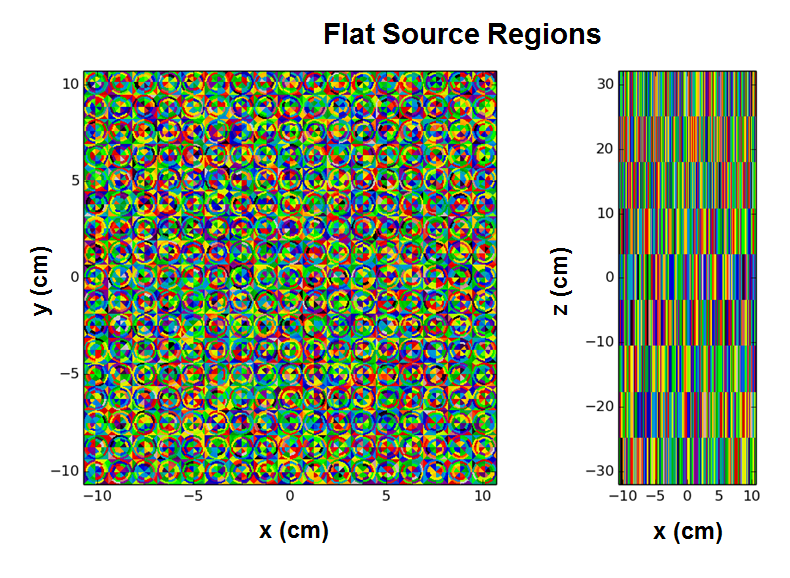
\includegraphics[width=0.75\linewidth]{figures/ph2016/fsrs.png}
	\caption{Flat source region discretization of the test problem. Pin cells are divided into 8 sectors with three rings in the fuel and two in the moderator, each with a height of 7.14 cm.}
	\label{fig::FSRs}
\end{figure}


\subsection{Performance Results}
Several cases were run on single AWS m4.10xlarge compute nodes using the different techniques described in this paper. The list of cases is given in Table~\ref{tab::cases}, ordered by their computational time for the eigenvalue calculation. 

\begin{table}[ht]
	\centering
	\caption{Descriptions for the ray tracing schemes tested in OpenMOC.}
	\begin{tabular}{c m{10cm}}
		\toprule
		\textbf{Case Number} & \textbf{Description} \\
		\midrule
		1 & On-the-fly stack ray tracing with temporary segment storage and local axial meshes \\
		2 & On-the-fly stack ray tracing with temporary segment storage and a global axial mesh \\
		3 & Explicit 3D segment storage \\
		4 & On-the-fly ray tracing by individual 3D track with a global axial mesh\\
		5 &On-the-fly ray tracing by individual 3D track with local axial meshes\\
		6 & On-the-fly stack ray tracing with direct MOC equations and local axial meshes \\
		7 & On-the-fly stack ray tracing with direct MOC equations and a global axial mesh \\
		\bottomrule
	\end{tabular}
	\label{tab::cases}
\end{table}


Note that the timing results do not include the time required to lay down 3D tracks or segment tracks before the beginning of the transport sweeps. Only the computational time to complete the 20 transport sweeps is counted. If the total run time were instead presented, explicit 3D segments would perform far worse since the time required to segment the tracks before the transport sweeps can be substantial. Still, the best on-the-fly methods actually outperform the explicit 3D segments in this study. A detailed description of the performance results for each case are presented in Tab.~\ref{tab::performance_results}.


\begin{table}[ht]
	\centering
	\caption{Computational results from the C5G7 single assembly test problem with several different ray tracing schemes in OpenMOC.}
	\begin{tabular}{ccc}
		\toprule
		\textbf{Case Number} & \textbf{Computation Time (s)} & \textbf{Total Memory (GB)} \\
		\midrule
		1  & 391.85 +/- 4.50 & 4.522 \\
		2  & 392.40 +/- 2.99 & 4.523 \\
		3  & 394.97 +/- 6.37 & 79.00 \\
		4  & 401.61 +/- 3.32 & 4.359 \\
		5  & 427.41 +/- 3.30 & 4.269 \\
		6  & 537.85 +/- 6.10 & 4.274 \\
		7  & 539.27 +/- 2.75 & 4.343 \\
		\bottomrule
	\end{tabular}
	\label{tab::performance_results}
\end{table}


The computational time for the different scheme was calculated by running each case 3 times on 6 different m4.10xlarge nodes. The median computational time was taken from each node and averaged across the six test nodes to provide the mean computation time and standard deviation, which was taken to be the uncertainty in the result. Total memory presented is the physical memory used by the OpenMOC.

Notice that the memory usage of explicit segmentation (case number 3) is more than an order of magnitude greater than the memory required for any of the on-the-fly axial ray tracing schemes. The computation times of the on-the-fly ray tracing schemes by $z$-stack with temporary segment storage are better than that with explicit segments, but the difference is well within the uncertainty associated with the results. The axial ray tracing schemes by individual 3D tracks are slightly slower, with the global axial mesh option being significantly faster than local meshes due to the lack of the need for a binary search on each new 2D segment. 

The axial ray tracing schemes by $z$-stack with direct application of the MOC equations perform the worst, likely due to the need for performing on-the-fly segmentation twice on each $z$-stack during a transport sweep. However, it is important to note that if higher order sources were added this scheme might become more attractive with more relative computational time being spent on applying the MOC equations to the track angular fluxes and FSR scalar fluxes than on actual ray tracing.

\begin{figure}[ht!]
	\centering
	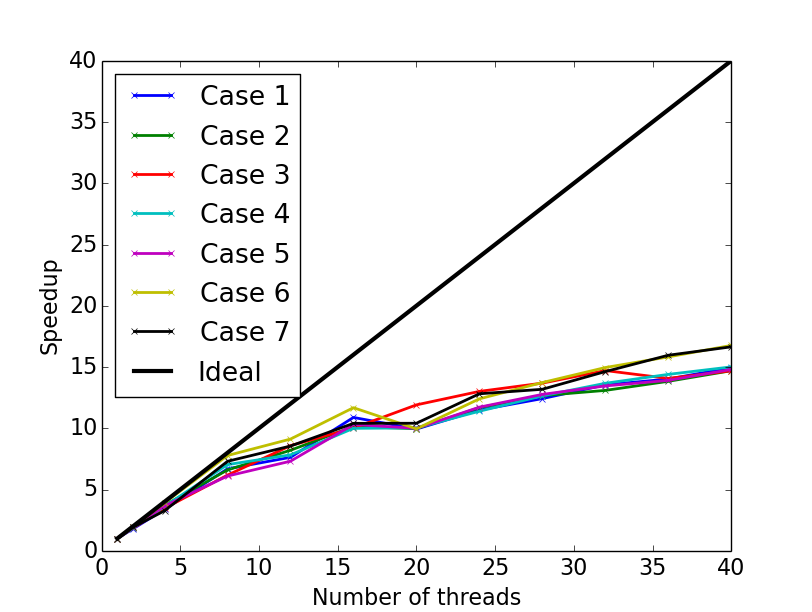
\includegraphics[width=0.75\linewidth]{figures/ph2016/scaling.png}
	\caption{Strong scaling results for the various ray tracing schemes on the C5G7 single assembly test problem.}
	\label{fig::scaling}
\end{figure}

Parallel scaling results are presented in Fig.~\ref{fig::scaling}. Notice that all the ray tracing schemes have similar parallel scaling performance during the transport sweeps. While the scaling is far from ideal, it is not saturated even at 40 cores. In more standard high performance computing, the scaling results would likely be far better, such as that observed for OpenMOC on BlueGene/Q\cite{will}.





%A description of this modified algorithm is presented in Algorithm~\ref{alg::new}.

%\begin{algorithm*}[!h]
%\caption{3D MOC algorithm extending the standard 2D approach}
%\label{alg::new}
%\begin{algorithmic}
%\STATE User specifies materials and a geometry
%\STATE Generate tracks across the geometry
%\STATE Create a superposition plane that contains all radial divisions
%\FORALL{$i \in \text{2D tracks}$}
%    \STATE Segment 2D track $i$ into 2D segments across the superposition plane, saving     the 2D segment lengths and corresponding axially extruded region identifiers,          populating the axially extruded regions as new regions are traversed
%\ENDFOR
%\FORALL{$A \in \text{axially extruded regions}$}
%    \STATE Create a vertical track in $A$ and segment the track through the 3D geometry, populating the 3D FSRs and saving their identifiers to $A$
%\ENDFOR
%\FORALL{transport sweeps}
%    \FORALL{$i \in \text{2D tracks}$}
%      \FORALL{$\theta \in \text{polar angles}$}
%        \FORALL{$t \in \text{z-stack for 2D track } i \text{ and polar angle } \theta$}
%           \FORALL{$s \in \text{2D segments for track } i$}
%               \STATE Determine the 3D segment on-the-fly by calculating whether a radial intersection defined by the 2D segment or an axial intersection defined by the axial mesh associated with $s$ is reached first
%                \STATE Apply Eq.~\ref{eq::fsr_attenuation} and Eq.~\ref{eq::scalar_flux} to track $t$ and the corresponding FSR
%                \ENDFOR
%            \ENDFOR
%        \ENDFOR
%    \ENDFOR
%    \IF{Source is converged} 
%        \RETURN
%    \ENDIF
%\ENDFOR
%\end{algorithmic}
%\end{algorithm*}




%------------------------------------------------------------------------------
%
%------------------------------------------------------------------------------
\section{CONCLUSION} 
\label{sect::conclusion}

In this study, an alternative approaches to 3D MOC were presented for segment storage whereby only 2D segments are stored and 3D segments are computed on-the-fly. This approach offers significant memory reduction with minimal or no computational overhead. Results show that the most efficient ray tracing tested was ray tracing entire $z$-stacks of 3D tracks with temporary storage of the computed segments.
\clearpage

\vfill
\begin{highlightsbox}[frametitle=Highlights]
\begin{itemize}
  \item The bias between OpenMC and OpenMOC is the result of the flux separability approximation which uses the scalar rather than the angular flux to collapse the total \ac{MGXS} in energy and space.
  \item The most rigorous solution would require the use of angular-dependent total \ac{MGXS}. However, most deterministic multi-group methods, including OpenMOC, are not equipped to use angular-dependent \ac{MGXS}.
  \item \ac{SPH} factors are introduced here as one approach to force reaction rate preservation in multi-group methods which use \ac{MC}-generated \ac{MGXS}.
  \item The \ac{SPH} factor scheme corrects the total \ac{MGXS} to enforce neutron balance with a reference fixed source computed from \ac{MC} tallies.
  \item The flux errors and eigenvalue bias between OpenMC and OpenMOC was largely resolved with \ac{SPH} factors for a 1D slab and 2D fuel pin.
  \item It is unclear if a generalizable scheme based upon \ac{SPH} factors may be used to correct for the flux separability approximation.
  \item Future work should investigate methods to account for the angular dependence of total \ac{MGXS} in order to adequately preserve reaction rates in fine-mesh transport methods with \ac{MC}-generated \ac{MGXS}.
\end{itemize}
\end{highlightsbox}
\vfill